\section{Desarrollo del diseño}
Inicialmente se hizo un recuento de los recursos disponibles para la realización del proyecto tanto software como hardware. El primer diseño consistía en un clúster utilizando contenedores Docker como host de los nodos de cómputo que serían desplegados en máquinas del laboratorio Waira como se ve en la figura \ref{fig:minihypatia}. Sin embargo, a lo largo de la implementación se descubrió que el software Slurm necesario para el clúster requería acceso a permisos de kernel los cuales eran muy complejos de otorgar para el alcance del proyecto. Debido a esto se replanteo el diseño ahora utilizando máquinas virtuales de Debian, creadas especialmente para minimizar el gasto de recursos ajenos a su funcionalidad, la implementación se puede ver en la figura \ref{fig:minihypatiadeb}. Este diseño nos permite más libertad a la hora de otorgar permisos a todos los diferentes componentes de software que hacen funcionar a nuestro clúster como slurm, munged y openMPI. Finalmente vimos la necesidad de registrar la información de los usuarios en un almacenamiento dedicado por lo que decidimos usar un NAS el cual tendría espacios de usuarios individuales

\begin{figure}[H]
    \centering
    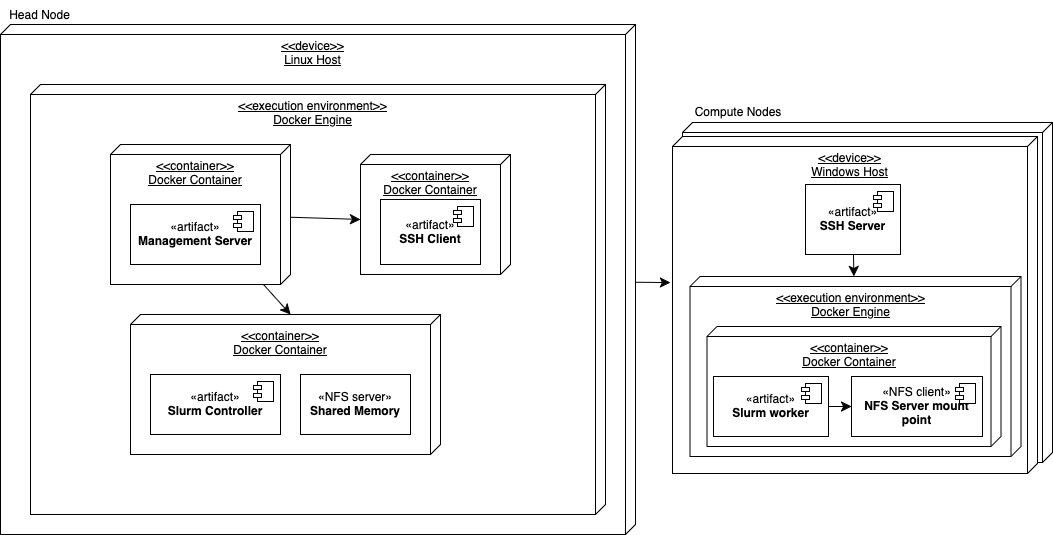
\includegraphics[width=0.75\linewidth]{Documento Final/Imagenes/MiniHypatia(1)-General Deployment.png}
    \caption{Diseño de Clúster UnaCloud con Docker}
    \label{fig:minihypatia}
\end{figure}

\begin{figure}[H]
    \centering
    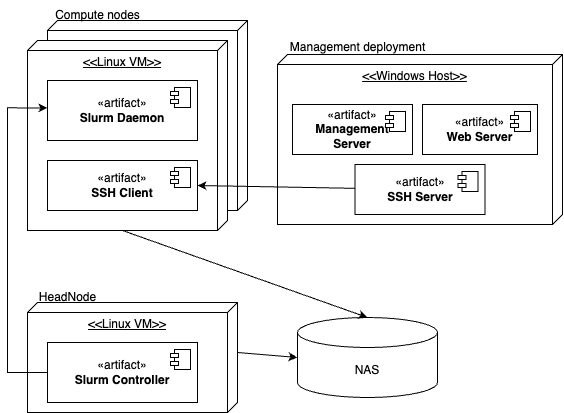
\includegraphics[width=0.75\linewidth]{Documento Final/Imagenes/dep.drawio.png}
    \caption{Diseño de Clúster UnaCloud con Debian}
    \label{fig:minihypatiadeb}
\end{figure}

\subsection{Recolección de Información}
Para el diseño del clúster HPC se recolecto información de las siguientes fuentes:
\begin{enumerate}
    \item  \textbf{Documentación de slurm: }La página web de documentación es un recurso muy importante. Ademas de hablar de las opciones y funcionamiento del software, hace recomendación sobre software que interactúa con este. Adicionalmente provee una guía muy detallada de cómo hacer el despliegue
    \item \textbf{ArchWiki: }A pesar de que no usamos la distribución Arch Linux, esta wiki contienen extensa información sobre diversas herramientas de software en linux además del funcionamiento del sistema operativo.
\end{enumerate}

\subsection{Alternativas de diseño}
Como se mencionó previamente se consideró bastante el uso de contenedores de Docker debido a su facilidad de arranque y portabilidad. Esa portabilidad también fue la razón por la que los terminamos descartando no están hechos con esta aplicación en mente. Otro componente alternativo fue la distribución, inicialmente se estaba usando Fedora sin embargo esta distribución tiene muchas aplicaciones instaladas por defecto, de las cuales muchas no necesitábamos, pero si consumían recursos tal como lo puede ser la GUI.
